%%%%% Set up %%%%%

% Set document style and font size
\documentclass[12pt]{article}\usepackage[]{graphicx}\usepackage[]{color}
%% maxwidth is the original width if it is less than linewidth
%% otherwise use linewidth (to make sure the graphics do not exceed the margin)
\makeatletter
\def\maxwidth{ %
  \ifdim\Gin@nat@width>\linewidth
    \linewidth
  \else
    \Gin@nat@width
  \fi
}
\makeatother

\definecolor{fgcolor}{rgb}{0.345, 0.345, 0.345}
\newcommand{\hlnum}[1]{\textcolor[rgb]{0.686,0.059,0.569}{#1}}%
\newcommand{\hlstr}[1]{\textcolor[rgb]{0.192,0.494,0.8}{#1}}%
\newcommand{\hlcom}[1]{\textcolor[rgb]{0.678,0.584,0.686}{\textit{#1}}}%
\newcommand{\hlopt}[1]{\textcolor[rgb]{0,0,0}{#1}}%
\newcommand{\hlstd}[1]{\textcolor[rgb]{0.345,0.345,0.345}{#1}}%
\newcommand{\hlkwa}[1]{\textcolor[rgb]{0.161,0.373,0.58}{\textbf{#1}}}%
\newcommand{\hlkwb}[1]{\textcolor[rgb]{0.69,0.353,0.396}{#1}}%
\newcommand{\hlkwc}[1]{\textcolor[rgb]{0.333,0.667,0.333}{#1}}%
\newcommand{\hlkwd}[1]{\textcolor[rgb]{0.737,0.353,0.396}{\textbf{#1}}}%
\let\hlipl\hlkwb

\usepackage{framed}
\makeatletter
\newenvironment{kframe}{%
 \def\at@end@of@kframe{}%
 \ifinner\ifhmode%
  \def\at@end@of@kframe{\end{minipage}}%
  \begin{minipage}{\columnwidth}%
 \fi\fi%
 \def\FrameCommand##1{\hskip\@totalleftmargin \hskip-\fboxsep
 \colorbox{shadecolor}{##1}\hskip-\fboxsep
     % There is no \\@totalrightmargin, so:
     \hskip-\linewidth \hskip-\@totalleftmargin \hskip\columnwidth}%
 \MakeFramed {\advance\hsize-\width
   \@totalleftmargin\z@ \linewidth\hsize
   \@setminipage}}%
 {\par\unskip\endMakeFramed%
 \at@end@of@kframe}
\makeatother

\definecolor{shadecolor}{rgb}{.97, .97, .97}
\definecolor{messagecolor}{rgb}{0, 0, 0}
\definecolor{warningcolor}{rgb}{1, 0, 1}
\definecolor{errorcolor}{rgb}{1, 0, 0}
\newenvironment{knitrout}{}{} % an empty environment to be redefined in TeX

\usepackage{alltt}

% File path to resources (style file etc)
\newcommand{\locRepo}{csas-style}

% Style file for DFO Technical Reports
\usepackage{\locRepo/tech-report}

% header-includes from R markdown entry
\usepackage{pdflscape}

%%%%% Variables %%%%%

% New definitions: Title, year, report number, authors
% Protect lower case words (i.e., species names) in \Addlcwords{}, in "TechReport.sty"
\newcommand{\trTitle}{Estimation of fork length using cranial measurements of sablefish (\emph{Anoplopoma fimbria}).}
\newcommand{\trYear}{2020}
\newcommand{\trReportNum}{nnn}
% Optional
\newcommand{\trAuthFootA}{Email: \href{mailto:Kathryn.Temple@dfo-mpo.gc.ca}{\nolinkurl{Kathryn.Temple@dfo-mpo.gc.ca}} \textbar{} telephone: (250) 756-7366}
\newcommand{\trAuthsLong}{Kathryn x. Temple, Lisa C. Lacko and Brendan M. Conners}
\newcommand{\trAuthsBack}{Kathryn x. Temple and Lacko, L.C. and Connors, B.M.}

% New definition: Address
\newcommand{\trAddy}{Pacific Biological Station\\
Fisheries and Oceans Canada, 3190 Hammond Bay Road\\
Nanaimo, British Columbia, V9T 6N7, Canada\\}

% Abstract
\newcommand{\trAbstract}{This document describes sampling activities and summarizes results}

% Resume (i.e., French abstract)
\newcommand{\trResume}{}

\newcommand{\trISBN}{}

%%%%% Start %%%%%

% Start the document
\IfFileExists{upquote.sty}{\usepackage{upquote}}{}
\begin{document}

%%%% Front matter %%%%%

% Add the first few pages
\frontmatter

%%%%% Drafts %%%%%

%\linenumbers  % Line numbers
%\onehalfspacing  % Extra space between lines
\renewcommand{\headrulewidth}{0.5pt}  % Header line
\renewcommand{\footrulewidth}{0.5pt}  % footer line
%\pagestyle{fancy}\fancyhead[c]{Draft: Do not cite or circulate}  % Header text

%%%%% Main document %%%%%
\hypertarget{introduction}{%
\section{Introduction}\label{introduction}}

Sablefish (\emph{Anoplopoma fimbria}) stock indices are derived from commercial and survey trap catch rates and estimates of trap vulnerable biomass determined from tag-recovery data. The tag and release study has been conducted annually since 1991. Whole tagged fish are recovered mainly in the commercial fishery (trap, trawl, hook and line) and processed at the point of landing through the Dockside Monitoring Program (DMP) currently operated by Archipelago Marine Research (AMR). In order to eliminate whole fish samples, we assessed whether sablefish fork length and weight could be predicted from 6 different head dimension measurements. Simple linear regression models were calculated from 438 sablefish (240-1080 mm) collected on 2 biennial DFO Groundfish Synoptic Bottom Trawl surveys in 2016 and one salmon survey (details).

\hypertarget{methods}{%
\section{Methods}\label{methods}}

\hypertarget{sample-collection-and-evaluation}{%
\subsection{Sample collection and evaluation}\label{sample-collection-and-evaluation}}

Measurements of fork length (FL), round weight (RW), upper jaw length (UJ), eye diameter (ED), interorbital distance (ID), snout length (SL), post orbital to preoperculum distance (PP), and post orbital head length (PH) were obtained from 212 sablefish caught during the 2016 West Coast Vancouver Island (WCVI) survey (Williams et al. \protect\hyperlink{ref-Williams2018}{2018}) and 219 sablefish caught during the 2016 West Coast Haida Gwaii (WCHG) survey (Nottingham et al. \protect\hyperlink{ref-Nottingham2018}{2018}) (Figure~\ref{fig:figure1}). Seven small sablefish were collected during the 201? (Kathryn) salmon survey. In addition, sagittal otoliths and operculum clips (DNA) were collected. Fish sex and maturity were recorded at sea (Table~\ref{tab:table1}).

The six cranial dimensions were considered as possible candidates for estimating fork length. Post orbital head lengths (PH) were abandoned after 130 fish due to measurement difficulties (Table~\ref{tab:table1}). Each of the 6 head dimensions were measured by Mitutoyo absolute 500-??? (Kathryn) digital calipers and ranked in terms of ease of use and repeatability. (Table~\ref{:table2}).

Later, a pilot study was conducted with the commercial sector returning sablefish heads, rather than the entire fish. In 2017, 360 heads were collected from J-cut sablefish on a trip to the Bowie Seamount. Each operculum was marked with either one knife cut (male) or two knife cuts (female) (Figure x) The first 99 heads of the pilot study were measured by 3 technicians for IO, SN, UJ and PP.

\hypertarget{genetic-test-development}{%
\subsection{Genetic test development}\label{genetic-test-development}}

DNA multiplex polymerase chain reactions (PCRs) were conducted using fluorescently labelled forward primers. X-insert and Y-insert specific primers developed by Rondeau et al. (\protect\hyperlink{ref-Rondeau2013}{2013}) were used, but the X-insert forward and Y-nested reverse were redesigned to produce slightly smaller PCR products.

\hypertarget{model-evaluation}{%
\subsection{Model evaluation}\label{model-evaluation}}

\hypertarget{discussion}{%
\section{Discussion}\label{discussion}}

Routine biological sampling procedures have been modified so that commercial fisheries are now only returning heads, rather than entire fish

\clearpage

\hypertarget{results}{%
\section{Results}\label{results}}

The mean values of the predictor and response variables (Table~\ref{tab:table2}).

Given the ease of measurement, we suggest that Interorbital distance be used to predict sablefish fork lengths and weights (Table~\ref{tab:table3}).

We found evidence of relationships between upper jaw length and fork length (p = \ensuremath{9.358\times 10^{-278}}) ; eye diameter and fork length (p = \ensuremath{5.34\times 10^{-203}}); interorbital distance and fork length (p = \ensuremath{5.539\times 10^{-272}} ); upper snout length and fork length (p = \ensuremath{4.593\times 10^{-292}}); postorbital to preoperculum length and fork length (p = \ensuremath{2.024\times 10^{-247}}); and postorbital head length and fork length (p = 0).

The estimated slope is 7.695 (SE 0.088) units of fork length per unit of upper jaw length; the estimated slope is 21.994 (SE 0.389) units of fork length per unit of eye diameter; the estimated slope is 11.622 (SE 0.138) units of fork length per unit of interorbital distance; the estimated slope is 11.182 (SE 0.118 units of fork length per unit of snout length; the estimated slope is 14.373 (SE 0.191) units of fork length per unit of postorbital to preoperculum length; and the estimated slope is 6.83 (SE 0.185) units of fork length per unit of postorbital head length.

\hypertarget{figures}{%
\section{Figures}\label{figures}}


\begin{figure}[htb]

{\centering \pdftooltip{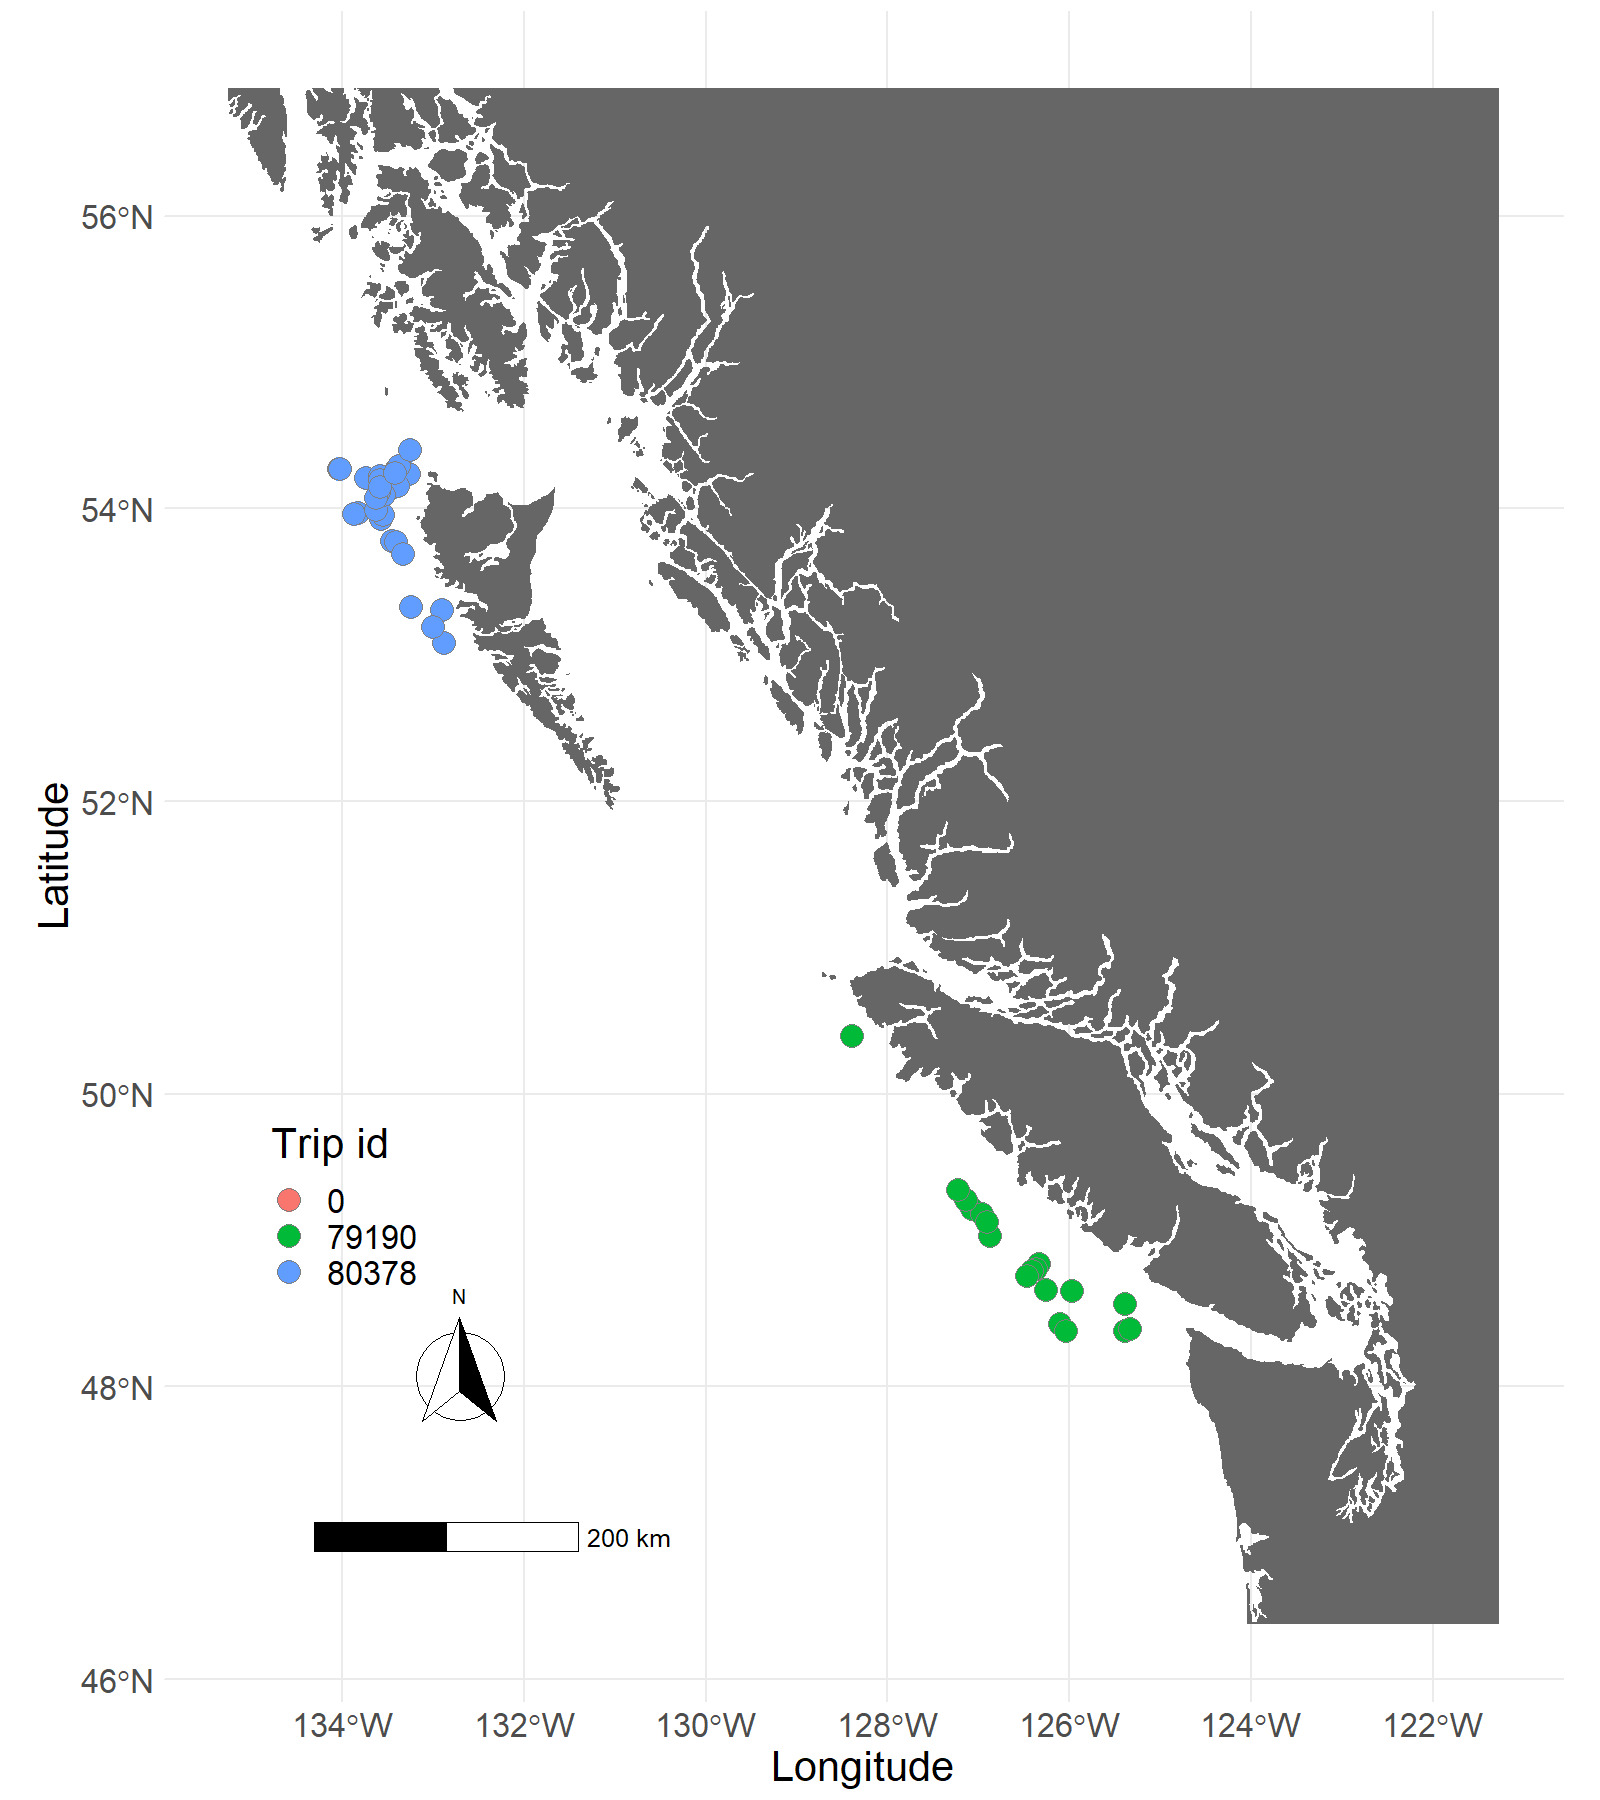
\includegraphics[width=6in]{C:/github/sablehead/figures/Figure1}}{Figure \ref{fig:figure1}} 

}

\caption{Sample locations.}\label{fig:figure1}
\end{figure}

\begin{figure}[htb]

{\centering \pdftooltip{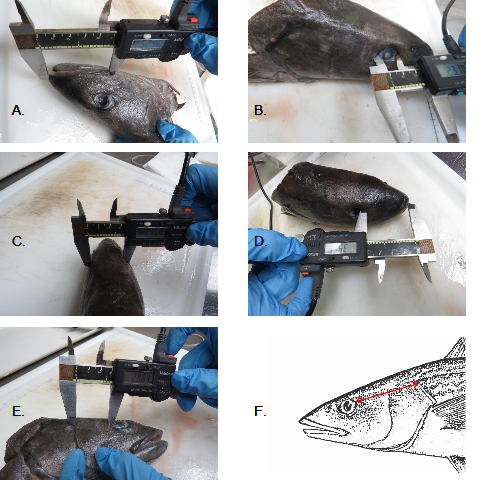
\includegraphics[width=6in]{C:/github/sablehead/figures/Figure2}}{Figure \ref{fig:figure2}} 

}

\caption{A. Upper jaw measurement; B. Eye diameter measurement; C. Interorbital distance; D. Snout length; E. Post orbital to preoperculum length measurement; F. Post orbital head length.}\label{fig:figure2}
\end{figure}

\begin{figure}[htb]

{\centering \pdftooltip{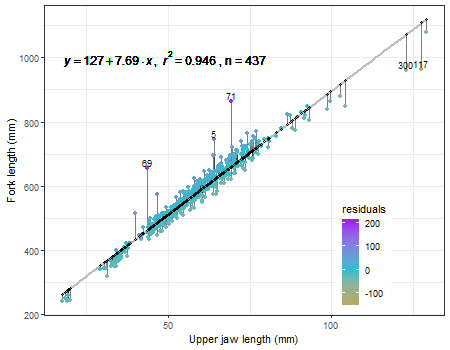
\includegraphics[width=400px,height=290px]{C:/github/sablehead/figures/Figure3}}{Figure \ref{fig:figure3}} 

}

\caption{Scatterplot upper jaw vs fork length, measurements in millimeters.}\label{fig:figure3}
\end{figure}

\begin{figure}[htb]

{\centering \pdftooltip{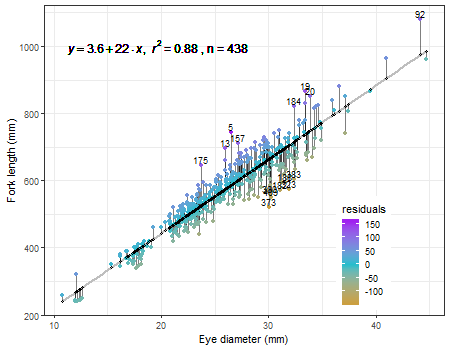
\includegraphics[width=400px,height=290px]{C:/github/sablehead/figures/Figure4}}{Figure \ref{fig:figure4}} 

}

\caption{Scatterplot eye diameter vs fork length, measurements in millimeters.}\label{fig:figure4}
\end{figure}

\begin{figure}[htb]

{\centering \pdftooltip{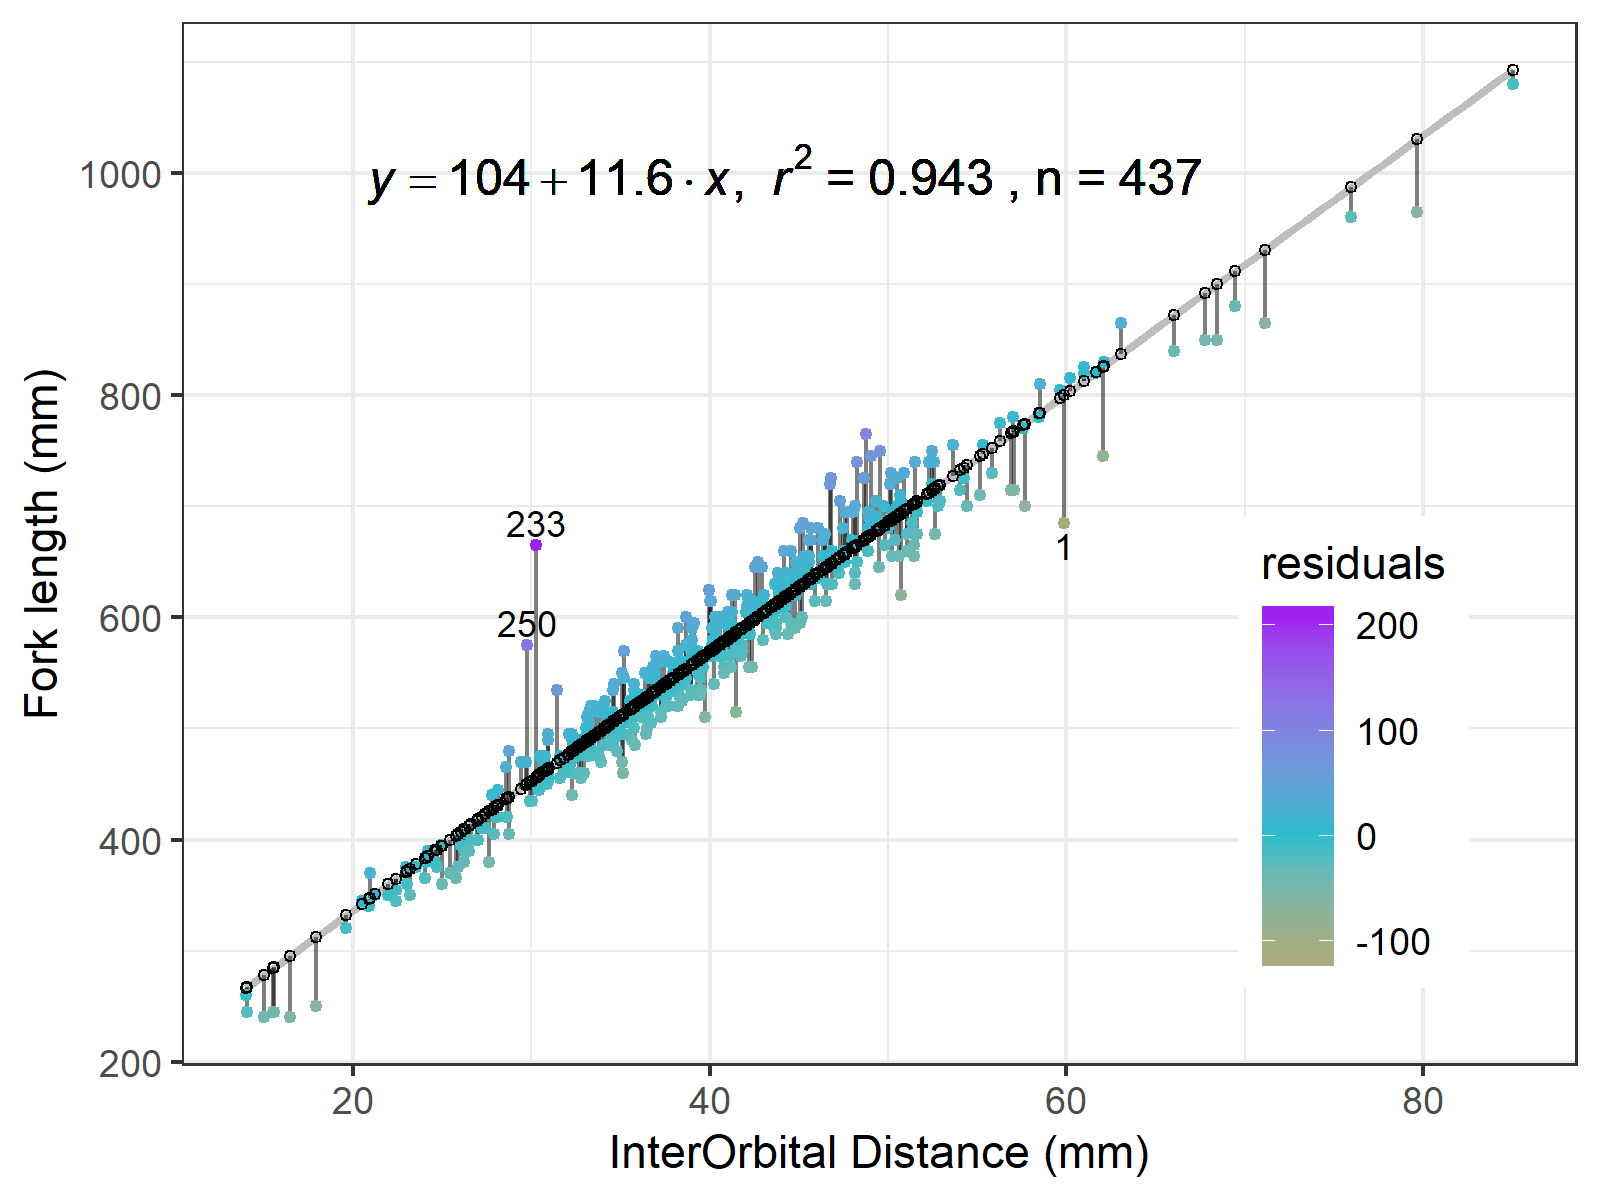
\includegraphics[width=400px,height=290px]{C:/github/sablehead/figures/Figure5}}{Figure \ref{fig:figure5}} 

}

\caption{Scatterplot interorbital vs fork length.}\label{fig:figure5}
\end{figure}

\begin{figure}[htb]

{\centering \pdftooltip{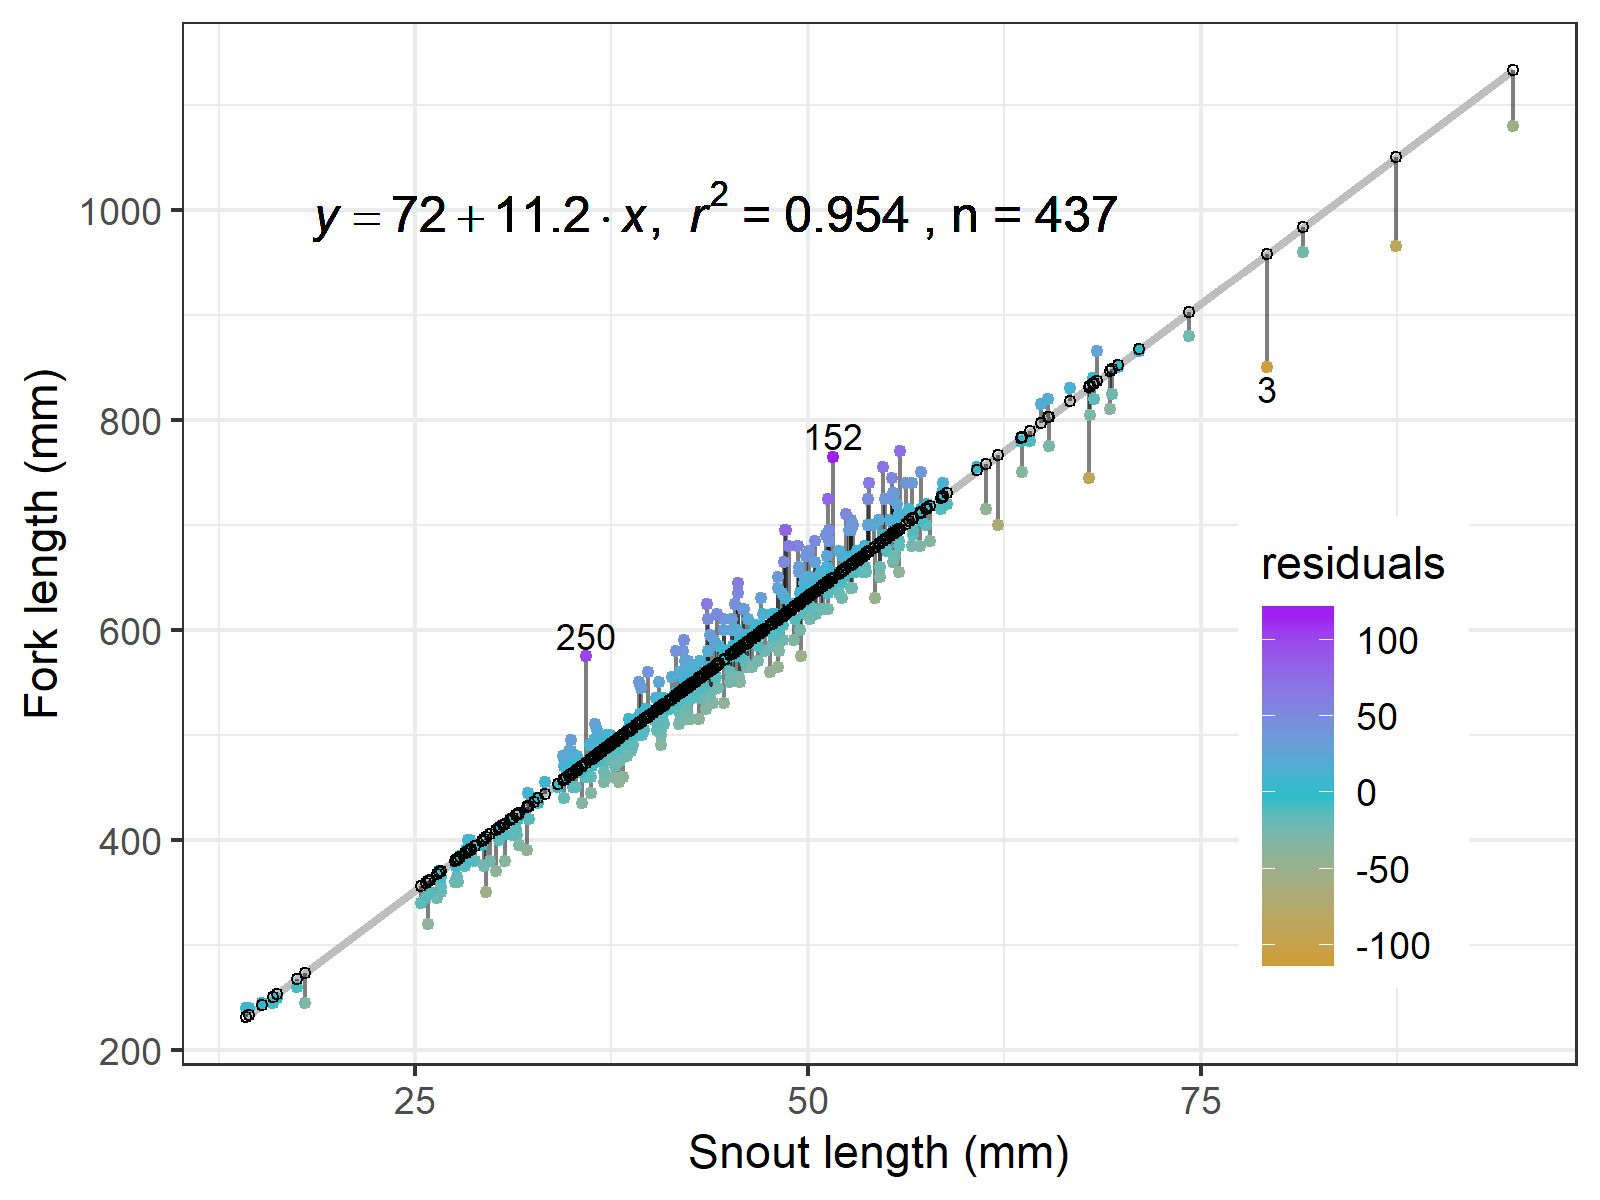
\includegraphics[width=400px,height=290px]{C:/github/sablehead/figures/Figure6}}{Figure \ref{fig:figure6}} 

}

\caption{Scatterplot snout length vs fork length.}\label{fig:figure6}
\end{figure}

\begin{figure}[htb]

{\centering \pdftooltip{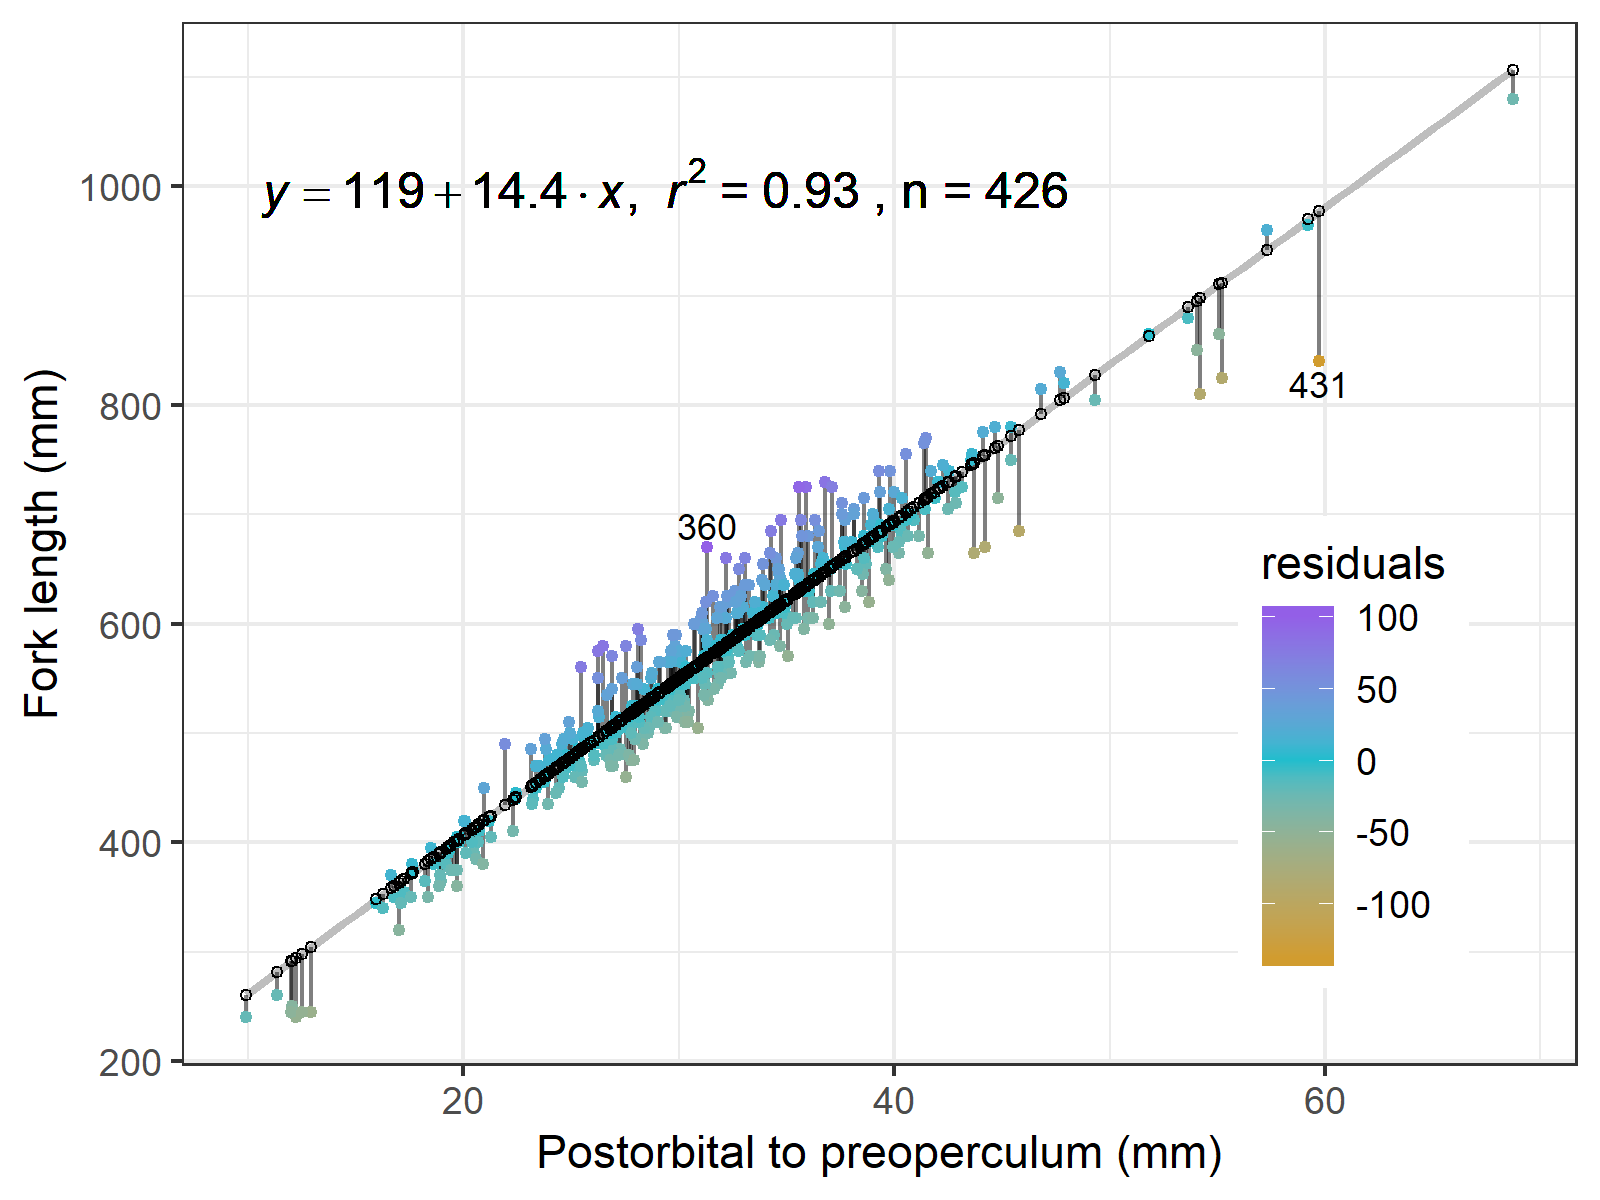
\includegraphics[width=400px,height=290px]{C:/github/sablehead/figures/Figure7}}{Figure \ref{fig:figure7}} 

}

\caption{Scatterplot post orbital to preoperculum length vs fork length.}\label{fig:figure7}
\end{figure}

\begin{figure}[htb]

{\centering \pdftooltip{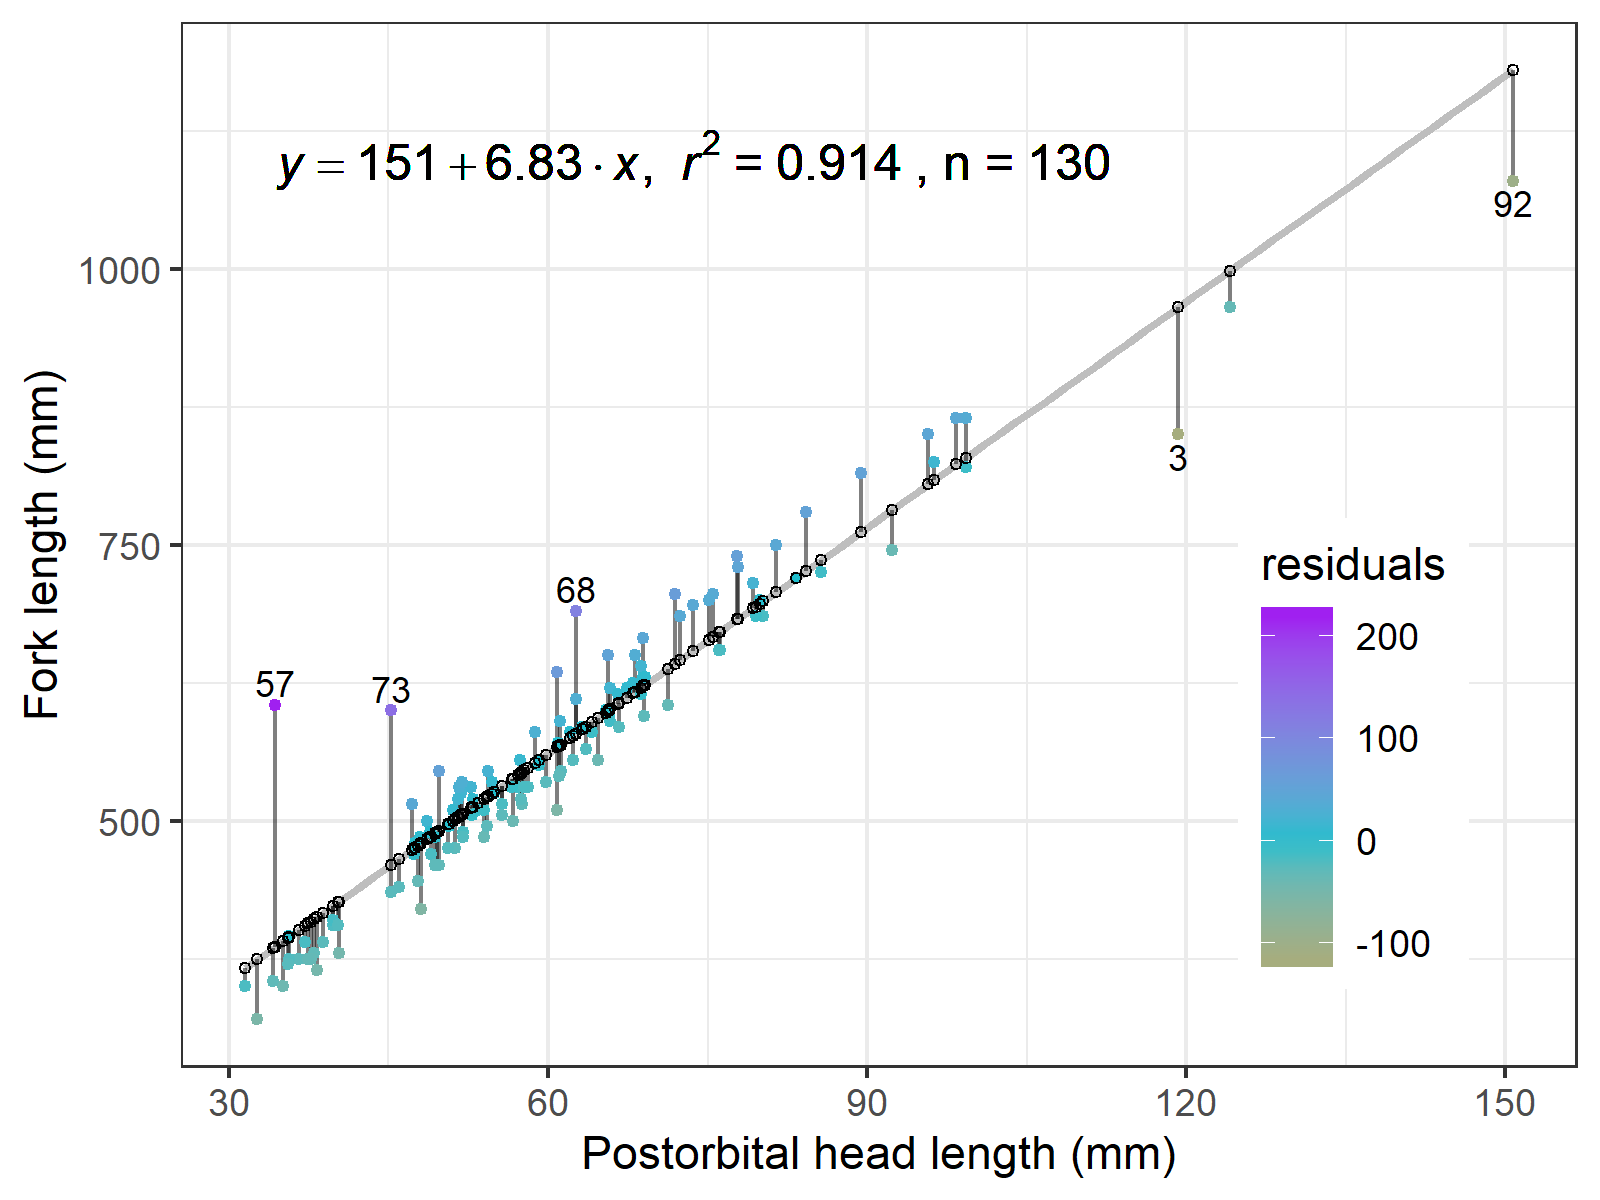
\includegraphics[width=400px,height=290px]{C:/github/sablehead/figures/Figure8}}{Figure \ref{fig:figure8}} 

}

\caption{Scatterplot of post orbital length vs fork length.}\label{fig:figure8}
\end{figure}
\clearpage

\hypertarget{discussion-1}{%
\section{Discussion}\label{discussion-1}}

Interorbial head length (IO) proved to be a good predictor of fork length for sablefish.

\hypertarget{acknowledgments}{%
\section{Acknowledgments}\label{acknowledgments}}

We thank \ldots{}

\hypertarget{refs}{}
\leavevmode\hypertarget{ref-Nottingham2018}{}%
Nottingham, M.K., Williams, D.C., Wyeth, M.R., and Olsen, N. 2018. Summary of the west coast haida gwaii synoptic bottom trawl survey, august 25 - september 26, 2016. Can. Manuscr. Rep. Fish. Aquat. Sci. 3151: viii: 51 p.

\leavevmode\hypertarget{ref-Rondeau2013}{}%
Rondeau, E.B., Messmer, A.M., Sanderson, D.S., Jantzen, S.G., Schalburg, K.R. von, Minkley, D.R., Leong, J.S., Macdonald, G.M., Davidsen, A.E., Parker, W.A., Mazzola, R.S.A., Campbell, B., and Koop, B.F. 2013. Genomics of sablefish (anoplopoma fimbria): Expressed genes, mitochondrial phylogeny, linkage map and identification of a putative sex gene. BMC Genomics 14(1): 452. Journal Article.

\leavevmode\hypertarget{ref-Williams2018}{}%
Williams, D.C., Nottingham, M.K., Olsen, N., and Wyeth, M.R. 2018. Summary of the west coast vancouver island synoptic bottom trawl survey, may 24 - june 15, 2016. Can. Manuscr. Rep. Fish. Aquat. Sci. 3137: viii: 54 p.
\end{document}
